

%%%%%%%%%%%%%%%%%%%%%%%%%%%%%%%%%%%%%%%%
%%%%%%%%%%%%%%%%%%%%%%%%%%%%%%%%%%%%%%%%
\section{Introduction}
%%%%%%%%%%%%%%%%%%%%%%%%%%%%%%%%%%%%%%%%
%%%%%%%%%%%%%%%%%%%%%%%%%%%%%%%%%%%%%%%%

%%%%%%%%%%%%%%%%%%%%%%%%%%%%%%%%%%%%%%%%
%%%%%%%%%%%%%%%%%%%%%%%%%%%%%%%%%%%%%%%%
\section{Methods}
%%%%%%%%%%%%%%%%%%%%%%%%%%%%%%%%%%%%%%%%
%%%%%%%%%%%%%%%%%%%%%%%%%%%%%%%%%%%%%%%%

\subsection{Extended pedigree data from older parents}

\subsection{Public data}
Previously published crossover data was obtained from the following sources:

\subsubsection{Oocytes}
\cite{Hou2013}
PB1(n=76), PB2(n=70), FPN(n=69)
Whole(n=215)
(MALBAC amplified)

\subsubsection{Sperm}
\cite{Wang2012} (Table S2 within \citet{Wang2012}. 2075 crossover events from 91 single sperm cells from the same individual, a 40 year old Caucasian male.)
MDA amplification, microarray: Illumina Omni1S Bead Array, but used previous sequencing results to confirm haplotypes.

\cite{Lu2012b} (pers. communication)
Sequenced 99 sperm cells from an Asian male (analyzed 91)
(MALBAC amplified)


%%%%%%%%%%%%%%%%%%%%%%%%%%%%%%%%%%%%%%%%
%%%%%%%%%%%%%%%%%%%%%%%%%%%%%%%%%%%%%%%%
\section{Results}
%%%%%%%%%%%%%%%%%%%%%%%%%%%%%%%%%%%%%%%%
%%%%%%%%%%%%%%%%%%%%%%%%%%%%%%%%%%%%%%%%
\subsection{23andMe data with older parents}


\begin{figure}[h]
    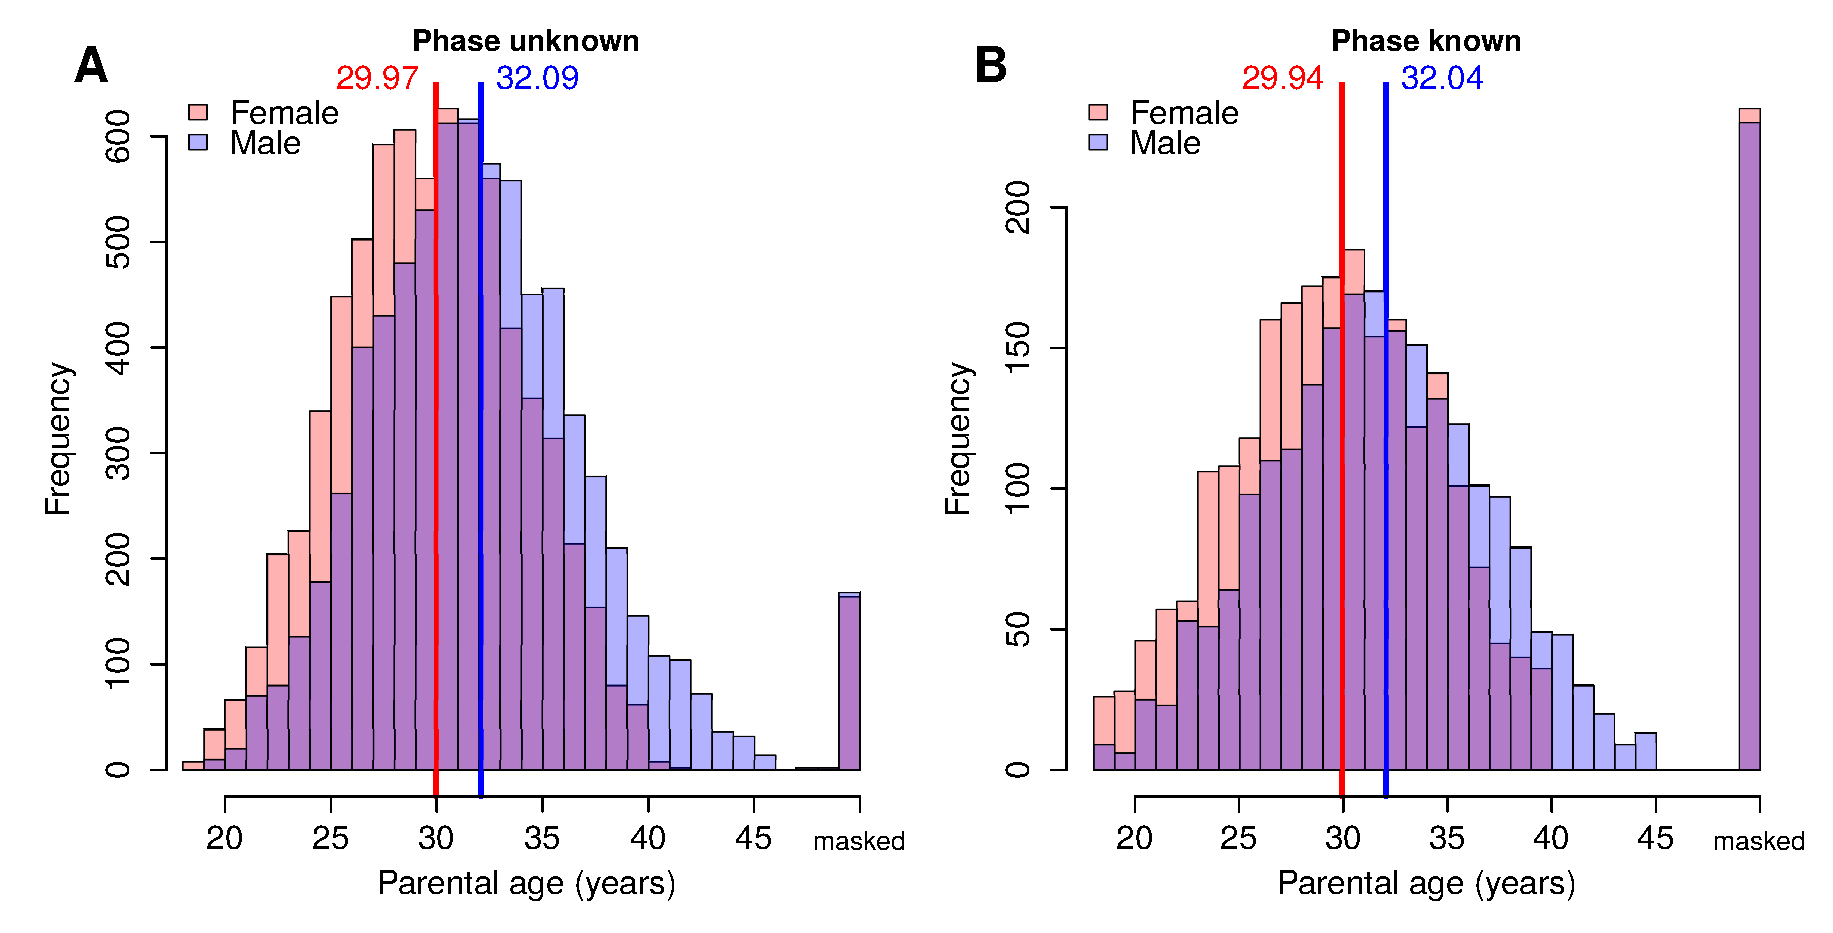
\includegraphics[width=\textwidth]{cointExtras/figs/ageHist_wMasked}
    \vspace{-20pt}
    \captionTitle{\textbf{Age distributions in the 23andMe dataset including older parents.}}{ 
        Phase-unknown parents are shown on the left panel (A), and phase-known parents, where ages were averaged across the children, are shown in the right panel (B).
        Additional data from older parents, in which the ages have been masked in females over 40 and males over 45 years old, are shown on the far-right of each distribution with the axis-label ``masked.''
        The vertical lines represent the mean of each distribution, excluding the older parents with masked ages.
    \label{fig:extrasAgeHist}}
\end{figure}

\subsection{Crossover interference}

\subsection{Maternal age effect}





\bibliographystyle{ccampbell_thesis} %unsrtnat} %abbrvnat_noURL} %abbrvUnsrt_last-first} %plain,unsrt,alpha,abbrv,acm,apalike,unsrt
\bibliography{/home/ccampbell/Dropbox/papers/thesis-cointExtras}
